\section{Smart Contracts}
\label{sec:smartContracts}
\secttoc

In this section we give further details of all the Solidity contracts, libraries and interfaces in the Nightfall repository.
Some of these contracts are pre-existing and some are new.
The important new contracts are:
\begin{itemize}
  \item Shield contract - stores `token commitments' which represent ownership of underlying ERC-20 or ERC-721 tokens, and facilitates the minting, transferring and burning of these token commitments.
  \item Verifier Contract - uses elliptic curve pairing functions to verify a zk-SNARK.
  \item Verifier Registry Contract - a registry of Verifier Contracts, Verification Keys, and Proof submissions. For simplicity, we ignore this layer from our explanations in this paper; although it is utilised in the Nightfall repository.
\end{itemize}

Here, we give further details of all Solidity contracts, libraries and interfaces in the Nightfall repository:\\
\\
\subsection{Pre-Existing Contracts}

\subsubsection{\texttt{ERC-721}}
The structuring of the ERC-721 contracts is aligned with the \url{https://0xcert.org} implementation.
These are designed for the transfer of non-fungible assets and include the following files:
\begin{center}
	\begin{tabular}{ll}
		\texttt{ERC721Interface.sol} & \\
		\texttt{ERC721TokenReceiver.sol} & \\
		\texttt{ERC721Metadata.sol} & \\
		\texttt{NFTokenMetadata.sol} & An example metadata implementation, to accompany \texttt{NFToken.sol} \\
		\texttt{NFToken.sol} & An example ERC-721 implementation.
	\end{tabular}
\end{center}
An overview of the ERC-721 contracts is given in Figure~\ref{pic:nftSmartContract}

\begin{figure}[H]
	\begin{center}
		\begin{mdframed}[backgroundcolor=black,userdefinedwidth=\textwidth,align=center]
			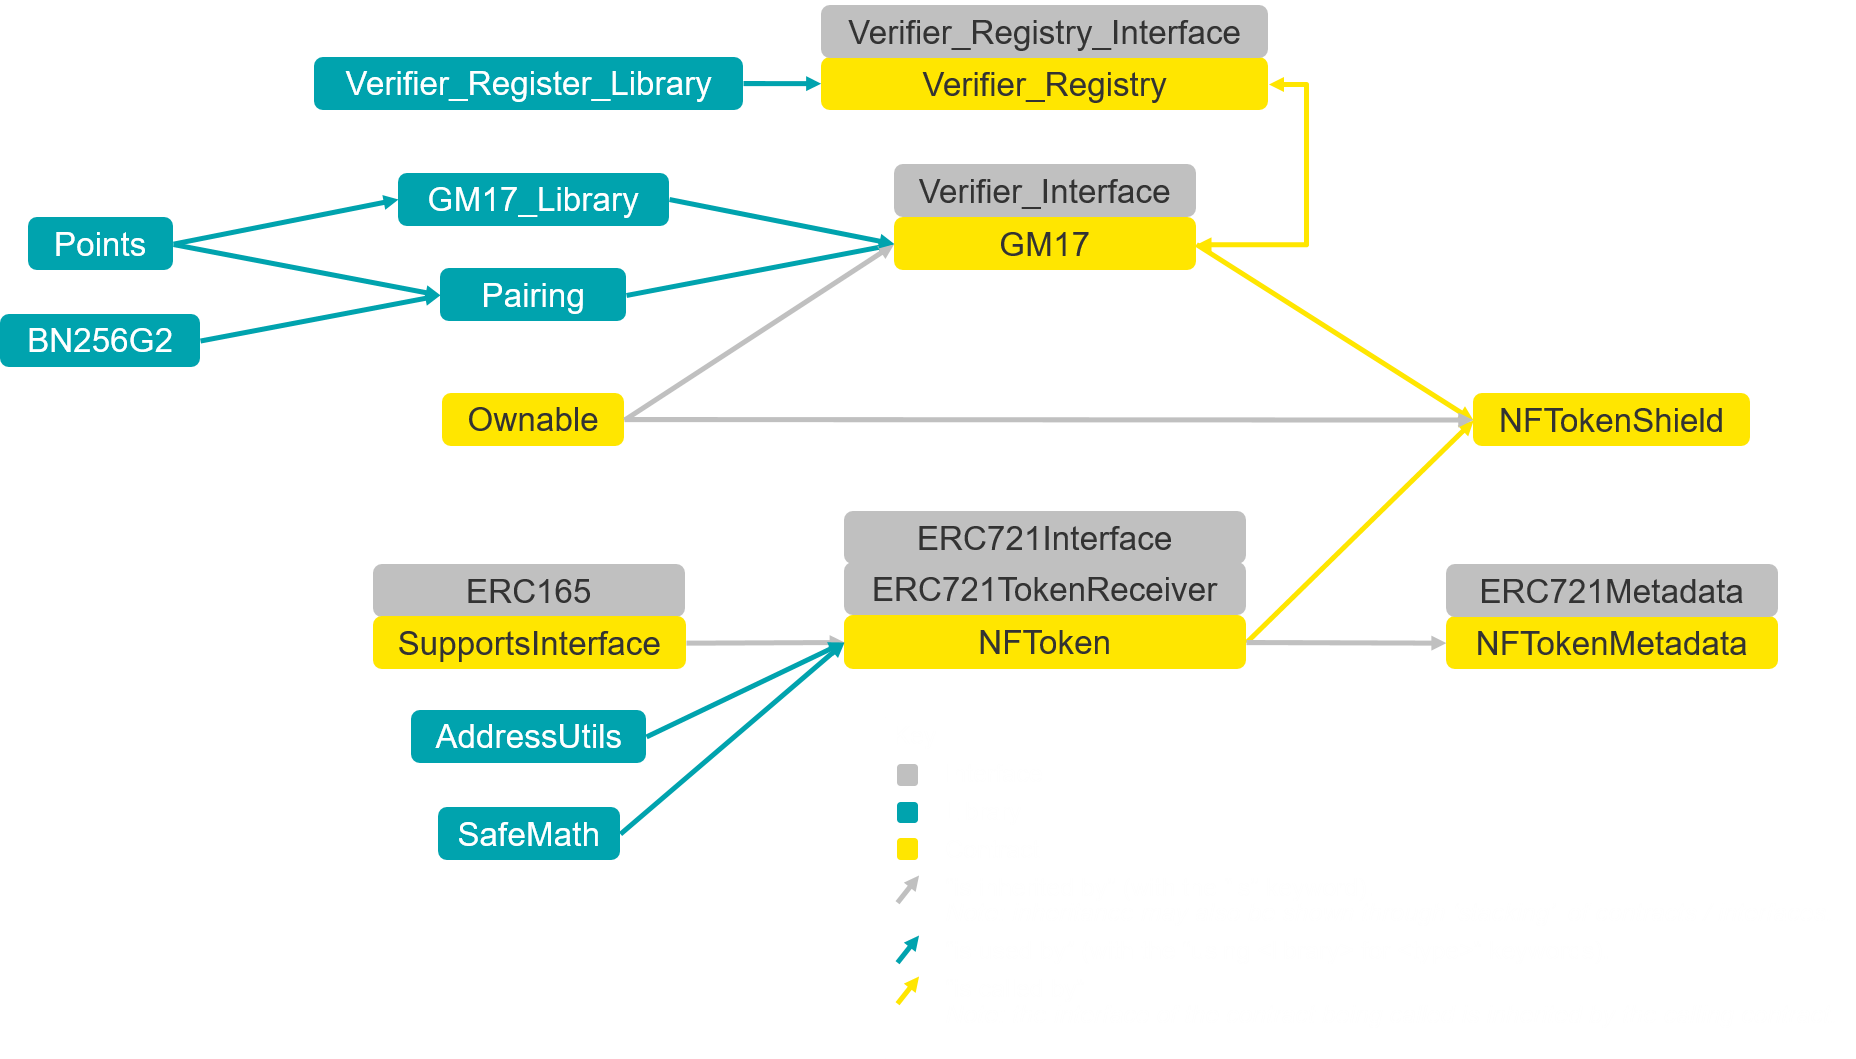
\includegraphics[width=\textwidth]{images/nft-contracts.png}
		\end{mdframed}
	\end{center}
	\caption{ERC-721 contract structure.}
	\label{pic:nftSmartContract}
\end{figure}

\subsubsection{\texttt{ERC-20}}
The structuring of the ERC-20 contracts is aligned with the \url{https://openzeppelin.org} implementation.
These are designed for the transfer of fungible assets and include the following files: 
\begin{center}
	\begin{tabular}{ll}
		\texttt{ERC20Interface.sol} & \\
		\texttt{FToken.sol} & An example ERC-20 implementation. \\
	\end{tabular}
\end{center}
An overview of the ERC-20 contracts is given in Figure~\ref{pic:ftSmartContract}

\begin{figure}[H]
	\begin{center}
		\begin{mdframed}[backgroundcolor=black,userdefinedwidth=\textwidth,align=center]
		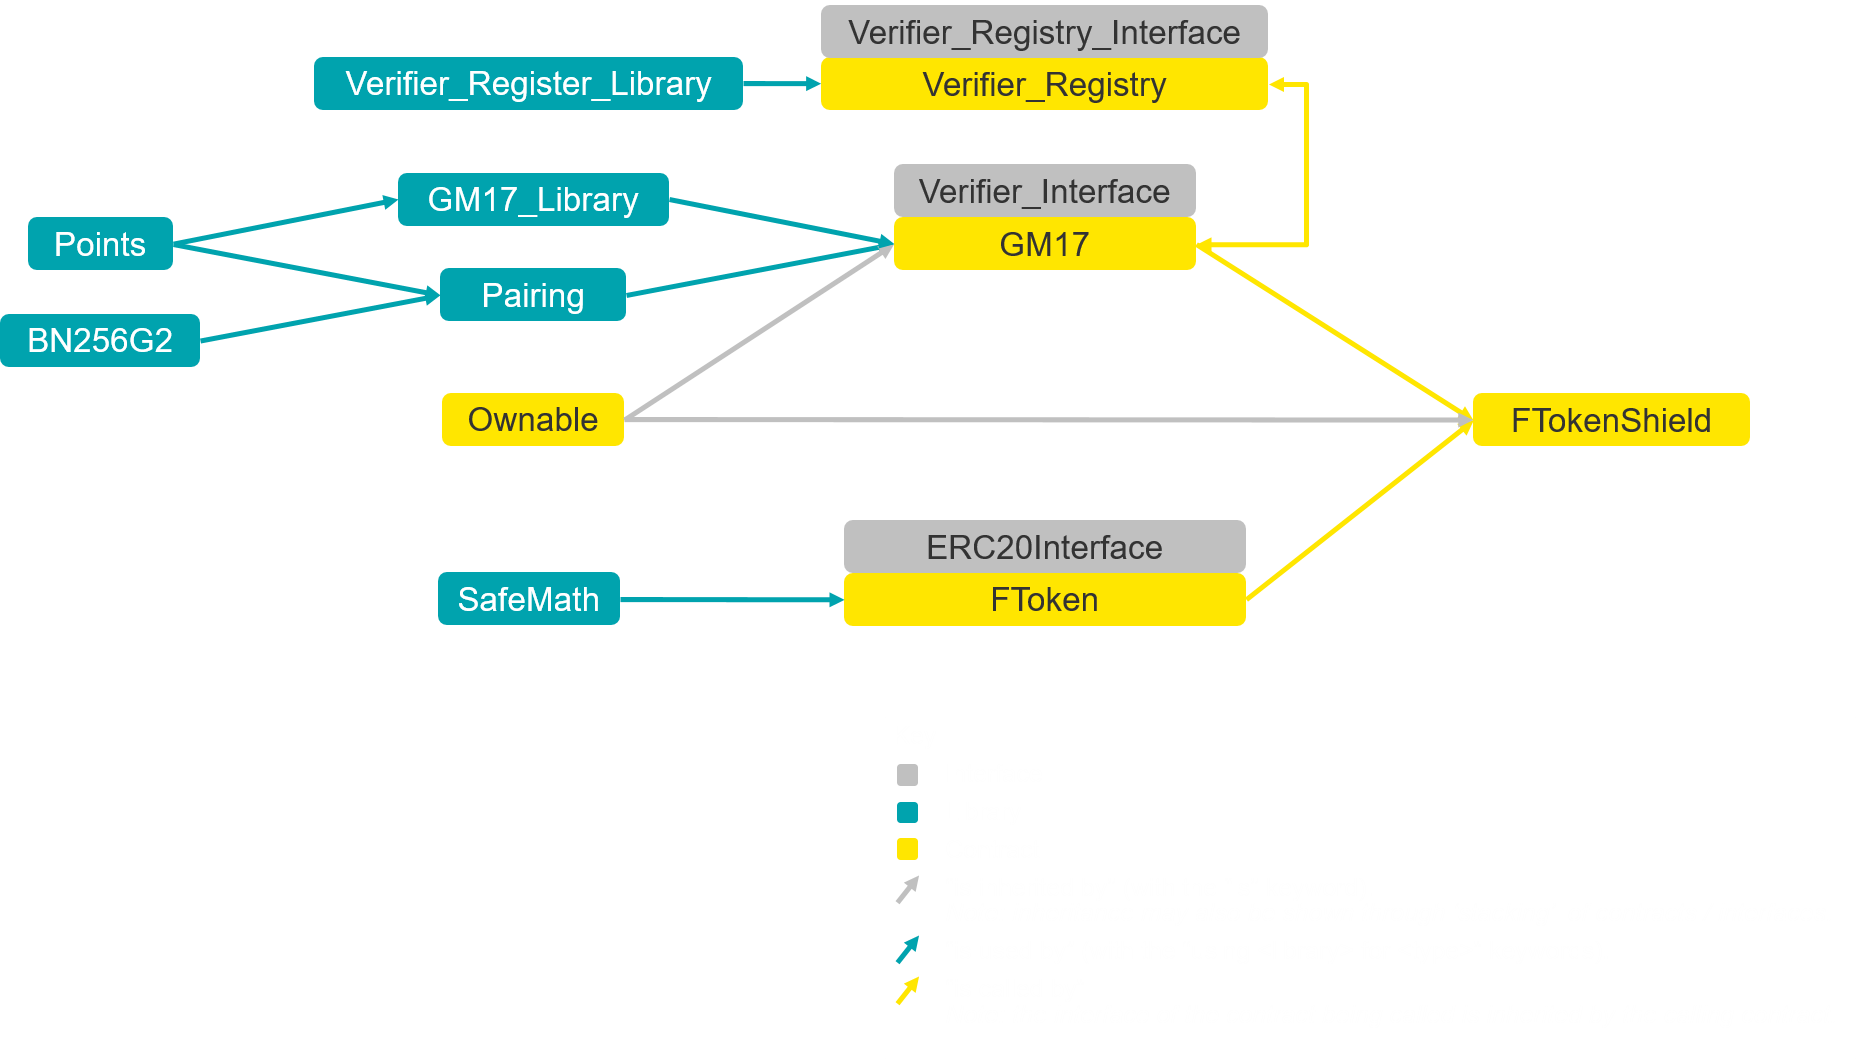
\includegraphics[width=\textwidth]{images/ft-contracts.png}
		\end{mdframed}
	\end{center}
	\caption{ERC-20 contract structure.}
	\label{pic:ftSmartContract}
\end{figure}

\subsubsection{\texttt{ERC-165}}
The structuring of the ERC-165 contracts is aligned with the \url{https://0xcert.org} implementation.
\begin{center}
	\begin{tabular}{ll}
		\texttt{ERC165Interface.sol} & \\
		\texttt{SupportsInterface.sol} &  \\
	\end{tabular}
\end{center}

\subsubsection{\texttt{Utility contracts}}
\begin{center}
	\begin{tabular}{ll}
		\texttt{AddressUtils.sol} & See \url{https://ethereum.stackexchange.com/a/14016/36603} for more details about how this works. \\
		\texttt{SafeMath.sol} & For safe mathematical operations.  \\
	\end{tabular}
\end{center}

\subsection{Shield contracts}
\subsubsection{\texttt{NFTokenShield.sol}}
Facilitates private transfers of Non-Fungible Tokens.

Constructor: At deployment, specify one Verifier contract (see below) and one ERC-721 contract. NFTokenShield will then be able to hold tokens of the ERC-721 contract in escrow, whilst the private counterparts of these tokens are transferred. Future contributions to Nightfall will produce an NFTokenShield contract which can handle multiple ERC-721 contracts at once.

Stores token commitments, which represent ownership of a token of the specified ERC-721 contract.

Calls upon the Verifier contract to verify zk-SNARKs for it.

A high-level diagram of the `shielding' process is shown in Figure~\ref{pic:nftShield}.

\begin{figure}[H]
	\begin{center}
		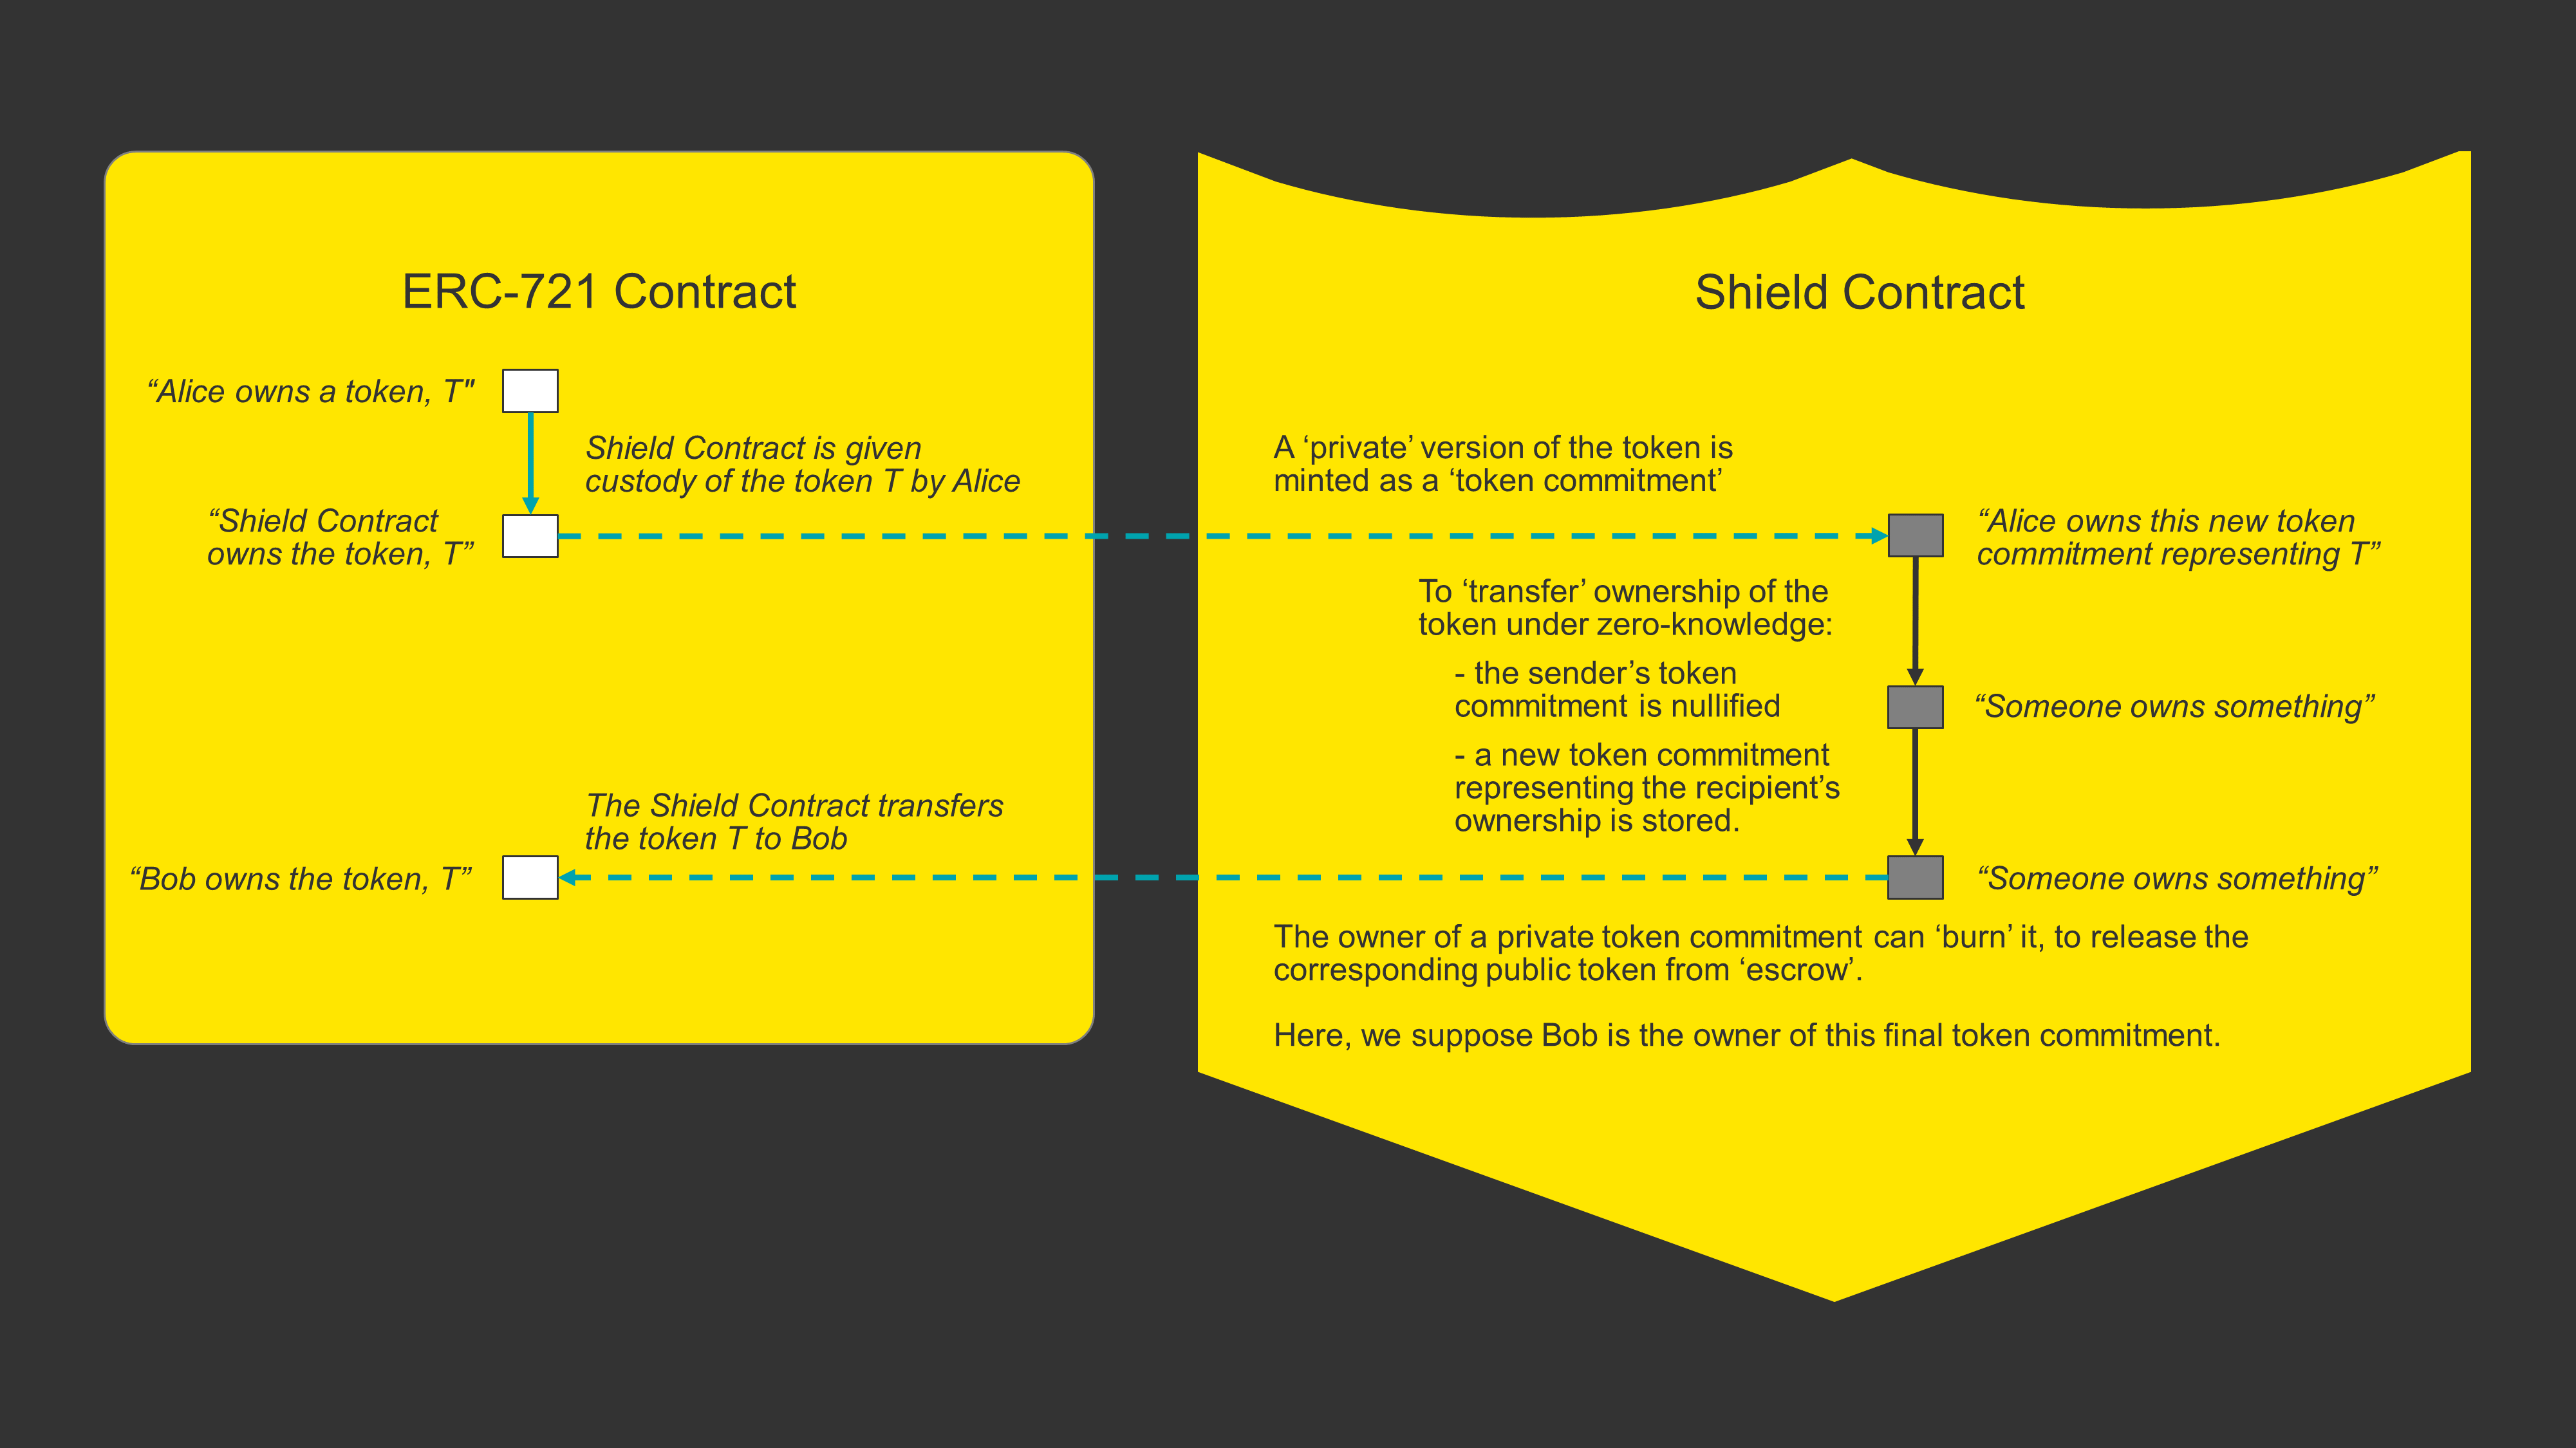
\includegraphics[width=\textwidth]{images/erc721Shielding.png}
	\end{center}
	\caption{High-level diagram of `shielding' an ERC-721 token.}
	\label{pic:nftShield}
\end{figure}

\subsubsection{\texttt{FTokenShield.sol}}
Facilitates private transfers of Fungible Tokens.

Constructor: At deployment, specify one Verifier contract (see below) and one ERC-20 contract. FTokenShield will then be able to hold tokens of the ERC-20 contract in escrow, whilst the private counterparts of these tokens are transferred. Future contributions to Nightfall will produce an FTokenShield contract which can handle multiple ERC-20 contracts at once.

Stores token commitments, which represent ownership of a particular amount of currency, as denominated in the specified ERC-20 contract.

Calls upon the Verifier contract to verify zk-SNARKs for it.

A high-level diagram of the `shielding' process is shown in Figure~\ref{pic:ftShield}.

\begin{figure}[H]
	\begin{center}
		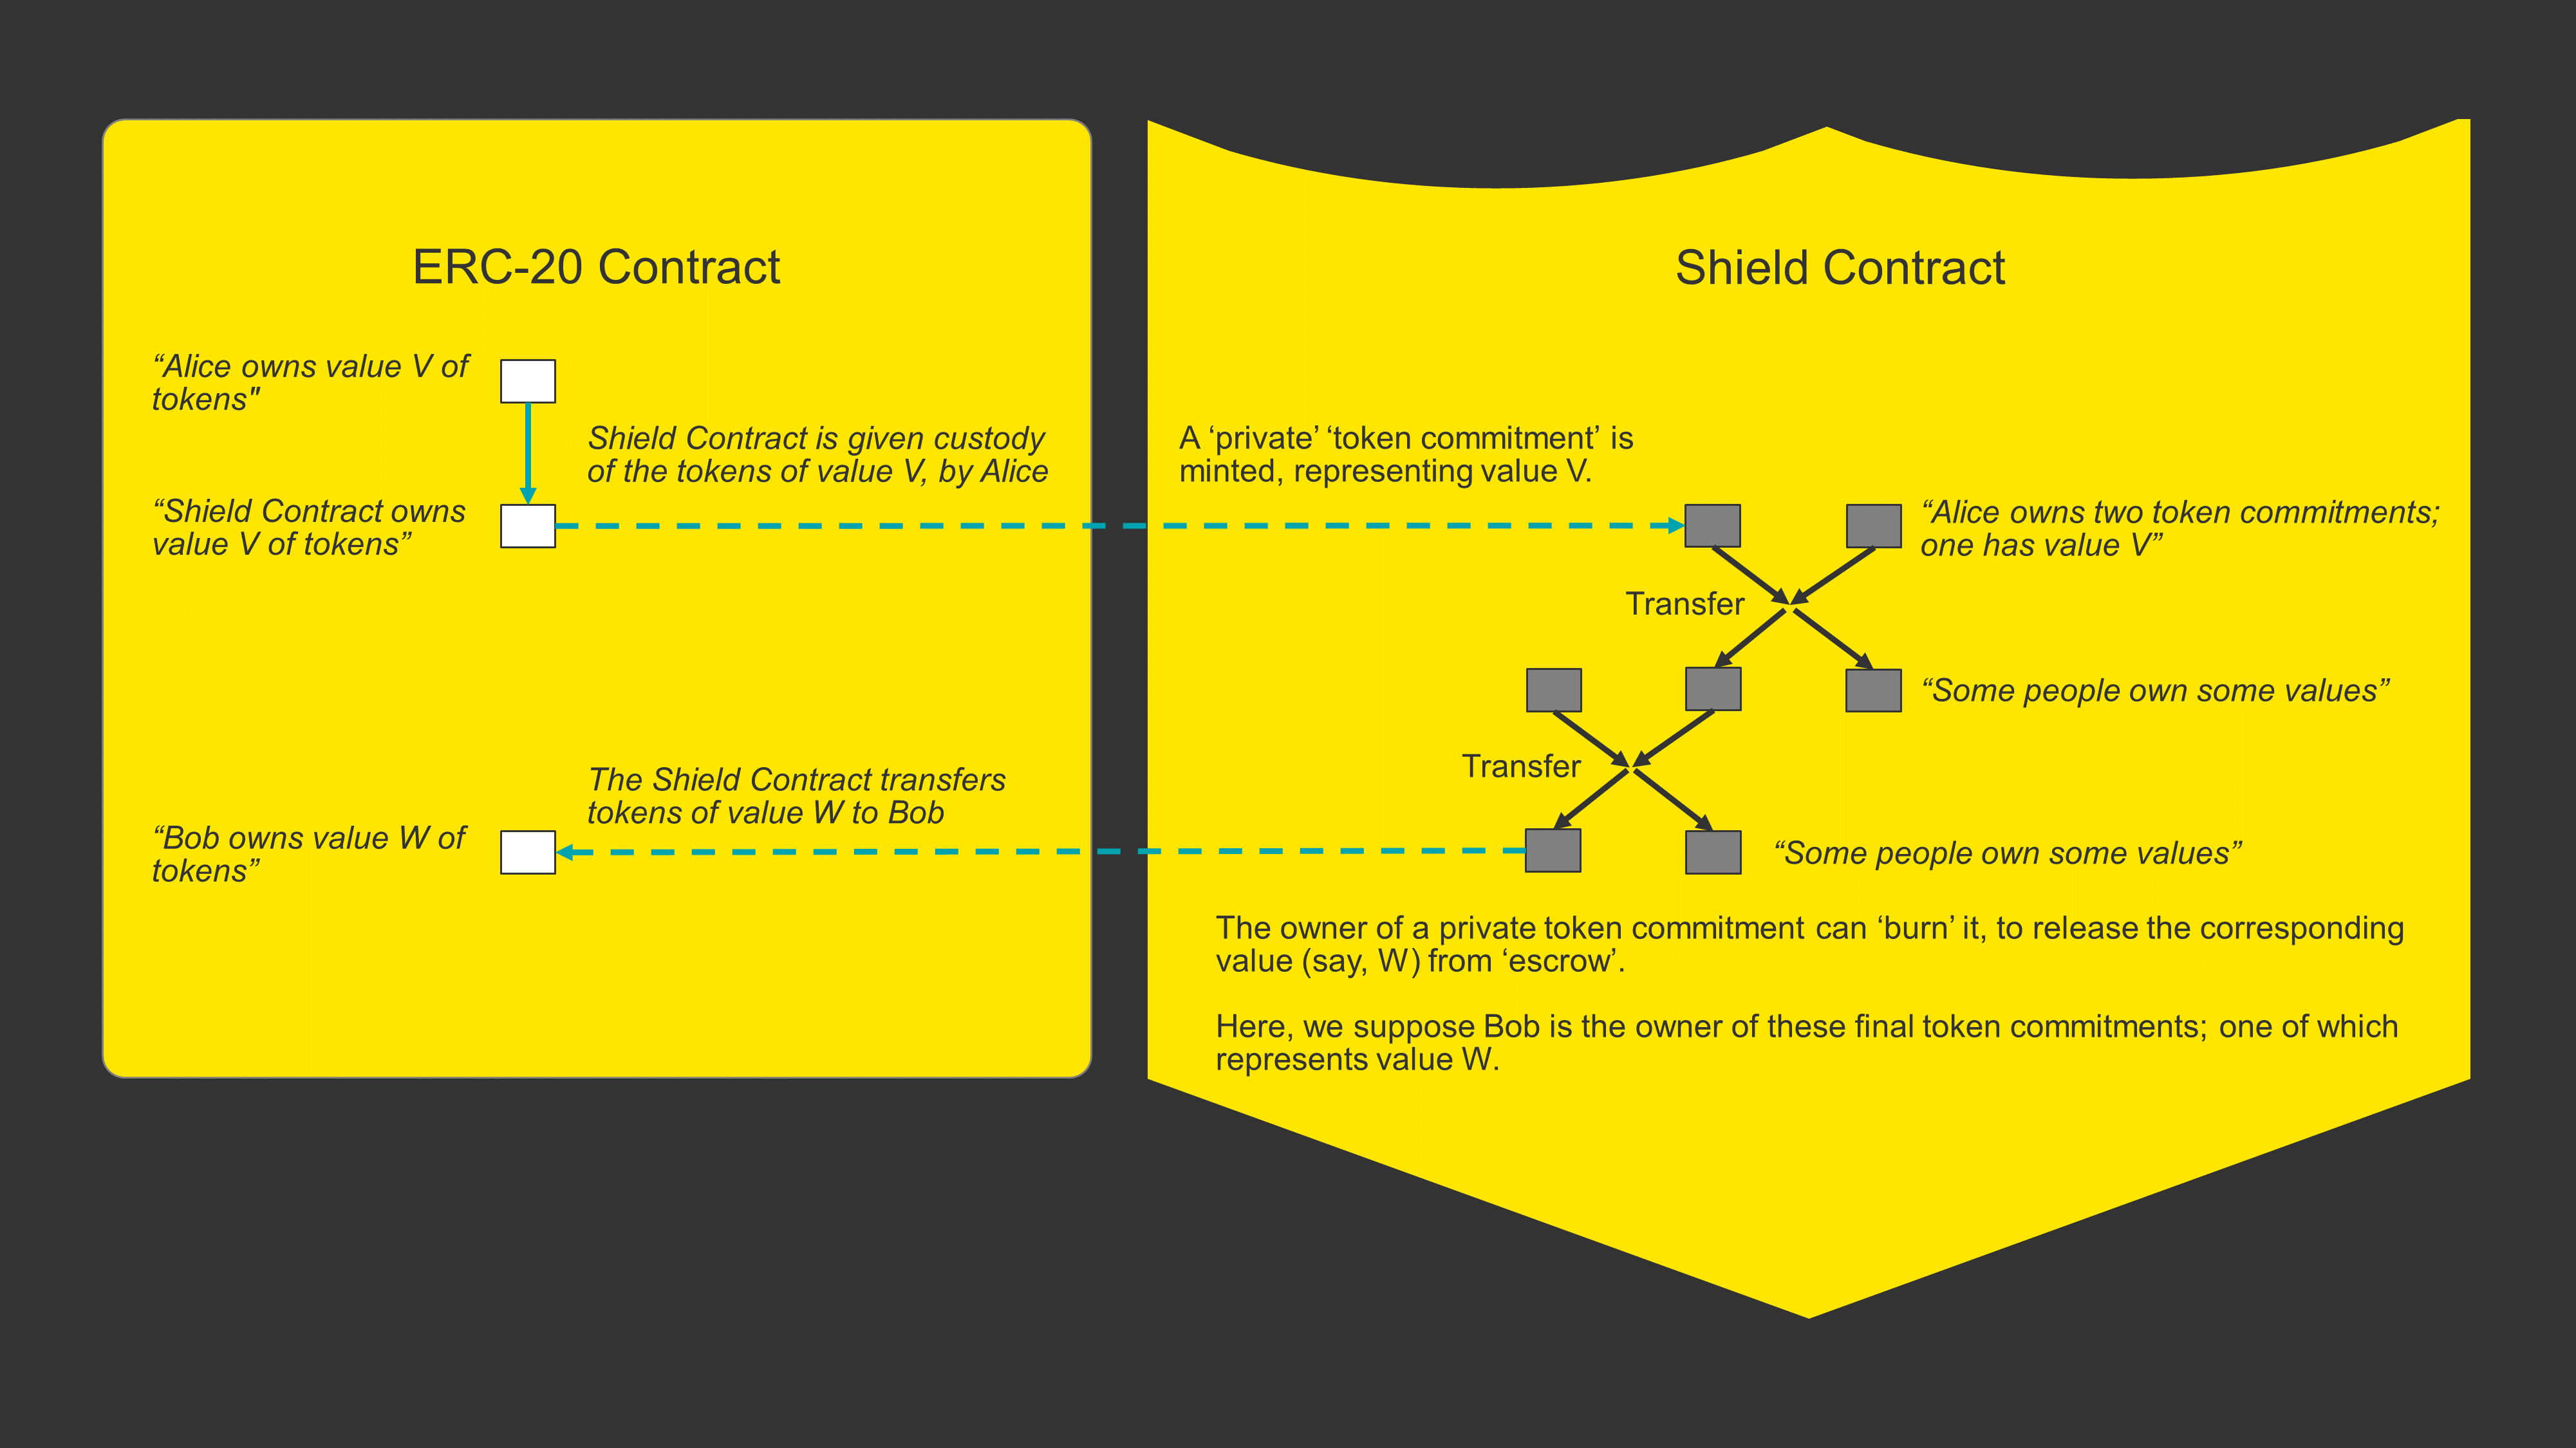
\includegraphics[width=\textwidth]{images/erc20Shielding.png}
	\end{center}
	\caption{High-level diagram of `shielding' an ERC-20 token.}
	\label{pic:ftShield}
\end{figure}

\subsection{Verifier contracts}
The sole purpose of a verifier contract is to verify zk-SNARKs which are passed to it. It returns \texttt{true} if the (proof, public inputs) pair verifies. Otherwise, it returns \texttt{false}.

\subsubsection{\texttt{GM17.sol}}
An implementation of the draft EIP-1922 zk-SNARK Verifier Standard. 

\subsubsection{\texttt{Points.sol}}
Library. Defines how Elliptic Curve coordinates $(x, y)$ are structured.

\subsubsection{\texttt{GM17Library.sol}}
Library. Defines the structures of both a Verification Key and a Proof under the GM17 protocol (using the elliptic curve points of \texttt{Points.sol}).

\subsubsection{\texttt{Pairing.sol}}
Library. Performs elliptic curve operations and elliptic curve pairing operations. Utilises the precompiled contracts of EIP-196 and EIP-197.

\subsection{Verifier Registry contracts}
The Verifier Registry is intended to be a single contract to register all zk-SNARK traffic on the Ethereum mainnet. It facilitates:
\begin{itemize}
  \item[--] Registration of Verifier contracts 
  \item[--] Storage of all Verification Keys
  \item[--] Proof submissions 
  \item[--] Other zk-SNARK use-cases beyond Nightfall 
\end{itemize}

Note: although the intention is for there to be just one Verifier Registry on the Ethereum mainnet, the default migration script in the Nightfall repository deploys an implementation of the Verifier Registry along with all other contracts -- for the sake of example.

\subsubsection{\texttt{Verifier\_Registry\_Interface.sol}}
The draft EIP-1923 interface for a Verifier Registry.

\subsubsection{\texttt{Verifier\_Registry.sol}}
An implementation of the Verifier\_Registry\_Interface.

\subsubsection{\texttt{Verifier\_Register\_Interface.sol}}
Library. Defines the structures of the register, which store entries to the Verifier\_Registry.

\subsection{Deployment of Contracts}
\label{sec:deploymentOfContracts}
See \hyperref[fig:trustedSetup]{Trusted Setup} for an explanation of deployment steps, and how contract deployment is intertwined with the zk-SNARK trusted setup.

\begin{center}
	\begin{mdframed}[backgroundcolor=verylightblue]
		Where to look?\\
		\\
		\begin{tabular}{lp{14cm}}
			\texttt{./zkp/contracts/} & Contracts in Nightfall\\
			\texttt{./zkp/migrations/} & Default deployment ordering of contracts in Nightfall\\
			\url{https://eips.ethereum.org/EIPS/eip-165} & EIP-165\\
			\url{https://eips.ethereum.org/EIPS/eip-20} & EIP-20\\
			\url{https://eips.ethereum.org/EIPS/eip-721} & EIP-721\\
			\url{https://eips.ethereum.org/EIPS/eip-196} & EIP-196\\
			\url{https://eips.ethereum.org/EIPS/eip-197} & EIP-197\\
			\url{https://eips.ethereum.org/EIPS/eip-1922} & EIP-1922\\
			\url{https://eips.ethereum.org/EIPS/eip-1923} & EIP-1923
		\end{tabular}
	\end{mdframed}
\end{center}




%Don't include figure until we get more. It looks out of place.
% \begin{figure}[H]
%   \centering
%   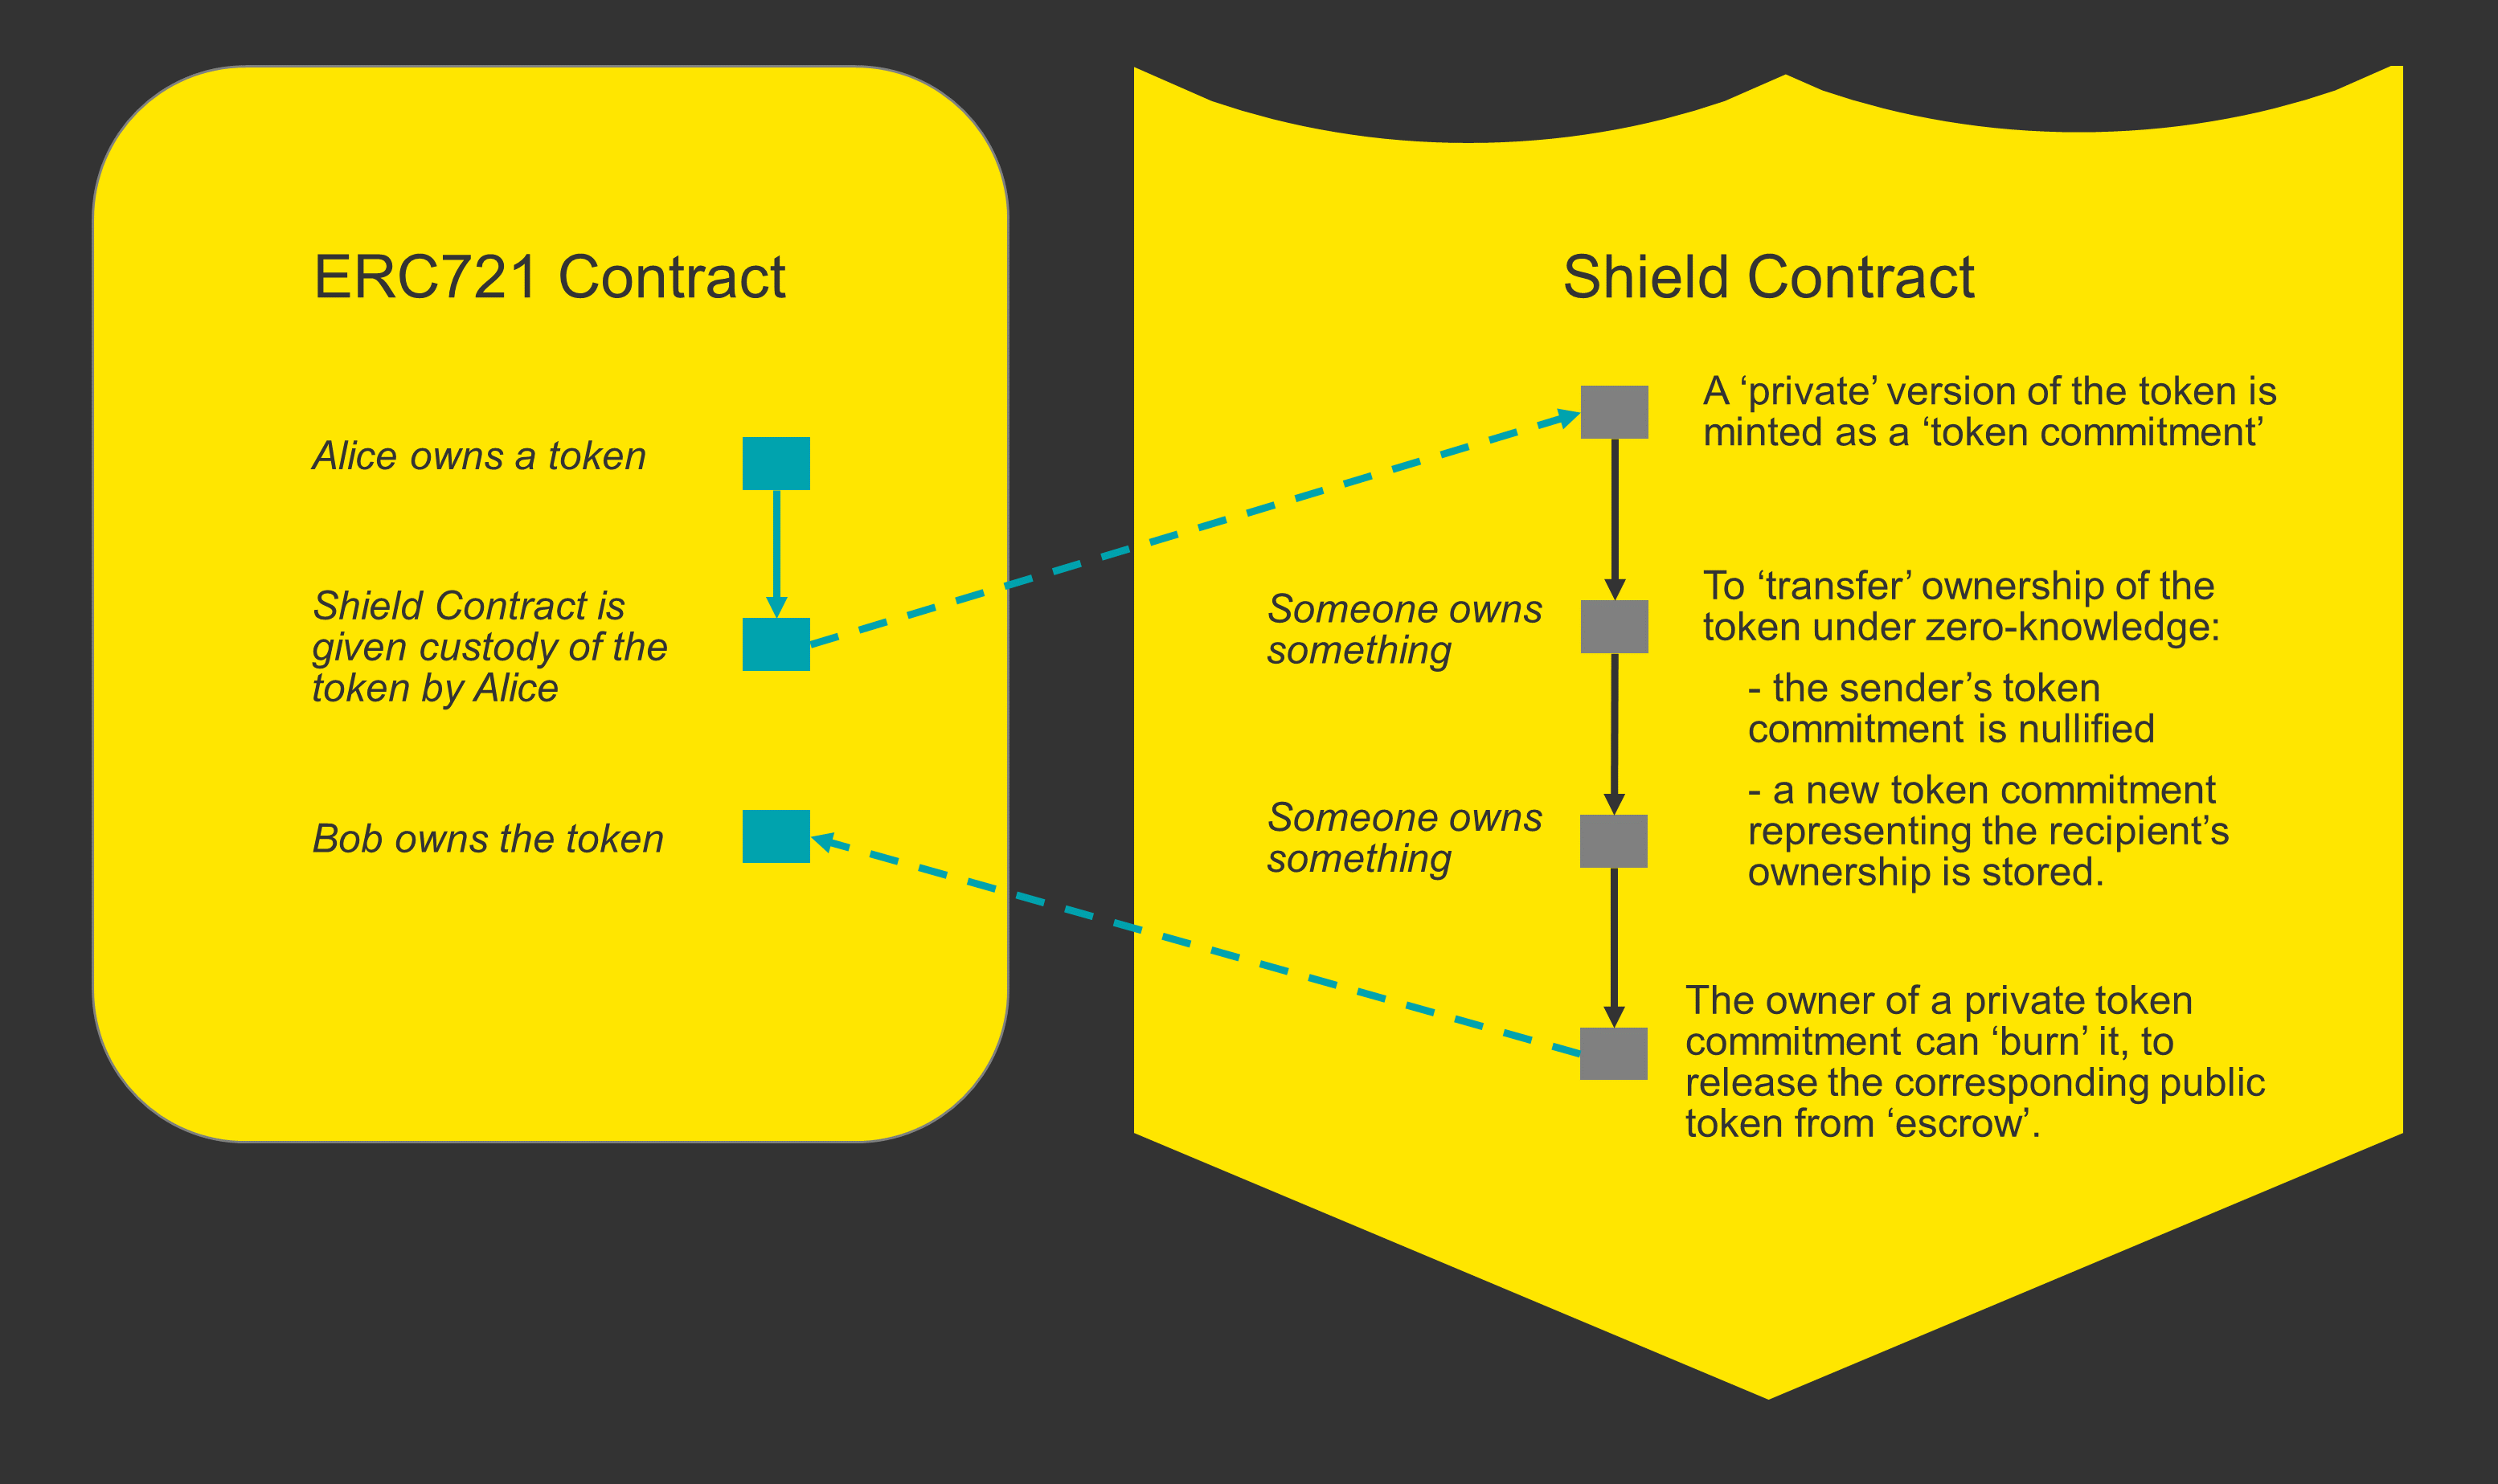
\includegraphics[scale=0.65]{smart-contracts}
%   \caption{The on-chain relationship between a `public' ERC-721 token and the `private' token commitments which represent it within the Shield Contract.}
%   \label{pic:Shield1}
% \end{figure}